\documentclass[11pt,conference]{IEEEtran}
\IEEEoverridecommandlockouts
% The preceding line is only needed to identify funding in the first footnote. If that is unneeded, please comment it out.
\usepackage{cite}
\usepackage{amsmath,amssymb,amsfonts}
\usepackage{algorithmic}
\usepackage{graphicx}
\usepackage{textcomp}
\usepackage{xcolor}
\def\BibTeX{{\rm B\kern-.05em{\sc i\kern-.025em b}\kern-.08em
    T\kern-.1667em\lower.7ex\hbox{E}\kern-.125emX}}
\begin{document}


\title{Conference Paper Title\\}

\author{\IEEEauthorblockN{Alessio Mina}
\IEEEauthorblockA{\textit{ETH Zurich, MSc Mech Eng}}
\and
\IEEEauthorblockN{Zelio Suter}
\IEEEauthorblockA{\textit{ETH Zurich, MSc Rsc}}
\and
\IEEEauthorblockN{Leon Züger}
\IEEEauthorblockA{\textit{ETH Zurich, MSc Mech Eng}}
}

\maketitle
\section{Introduction}

Misinformation represents a considerable threat for various aspects in our society. First of all, it represents one of the greatest threats for democracy and journalism\cite{Zhou2019}. Fake news are more shared on social media than real news, as it has been seen in US 2016 presidential elections\cite{Zhou2020}. Swiss security policy report 2021\cite{swiss2021} and US national intelligence global trends 2040 report \cite{us2021} remark that misinformation represents a threat for global security and stability: both reports foresee an increase of hybrid conflicts with misinformation and cyber offensive. Misinformation may also have a strong influence on our economy. For example, a false report of United Airlines parent company's bankruptcy in 2008 cause the company's stock price to drop by 76$\%$ in a few minutes\cite{carvalho2011}. Fake news can also have tremendous effects on public health, if one consider for example the misinformation around vaccines\cite{Larson2017}. Finally, as it has been shown for Japan earthquake in 2011\cite{Hashimoto2021}, reliable news sources are crucial during catastrophes, to avoid widespread of panic or criminal activities.\\

For all these reasons, it is important to study how misinformation spread among a society. Today context, with internet and social media representing a powerful vector for spreading fake news, and the trend of many people gravitating toward familiar and like-minded groups which are more likely to be in conflict, is particularly favourable for misinformation and opinion polarization\cite{us2021}. The goal of this paper is applying distributed systems theory to opinion dynamics in a society and study the spread of misinformation. In particular, we want to develop a model to investigate different scenarios and which factors influence the consensus or the opinion distribution type (ex. consensus or polarization).
Identifying misinformation spread dynamic is crucial to mitigate negative consequences with specific measures such as instruction level\cite{joanna2017} or social network intervention\cite{mahak2020}.


\subsection{Related Literature}

Misinformation spreading has been widely studied, above all in recent years with the rise of social media. An exhaustive literature review is beyond the scope of this work.\\

A two-stage process to model the spread of fake news on twitter is proposed in \cite{Murayama2021}. \cite{Rath2019} investigates the role community structures play in the spread of fake news, using an epidemiological model approach. An epidemiological model is also used by \cite{Tambuscio2015} to analyzed the spread of misinformation. \cite{Hashimoto2021} uses graph theory to study how the truthfulness of a topic influences the opinion dynamics and how it changes after a disaster. \cite{Amelkin2017} also studies a polar opinion dynamic in social network and introduce a metric to quantify the opinion propagation. The relation between social media, network heterogeneity and opinion polarization is the focus of \cite{Lee2014a} and shows that the use of social media is a predictor of network heterogeneity. In our work, we also investigate opinion polarization using the model developed. There is not a unique definition of polarization and \cite{Bramsona2016} exposes 9 different definitions of polarization with the corresponding measure. Also \cite{Akoglu2014} and \cite{Matakos2017} propose a metric to quantify polarization and effective strategies to reduce it. Moreover, the dynamic of polarization is investigated in \cite{Banisch2019}, in particular how it changes with social feedback, and in \cite{Conover2011}, where is analyzed how social media facilitate communication between communities with different political orientations. In addition to the contributions above, measures to mitigate fake news spread are studied from different points of view. \cite{mahak2020} develops a social reinforcement approach to combat the spread of fake news with an intervention model. Fake news detection has also been widely studied, for example in \cite{Vijjali2020}\cite{improved}\cite{Zhou2020}\cite{Maryam2019}. Other combat strategies rely on instruction and critical thinking \cite{joanna2017}.


\section{Statement of Contribution}

DA FARE ALLA FINE
\section{Mathematical Formulation}
\label{sec:mathematical}
To study the spread of news in the population, three types of agents are considered: individuals (also called "people"), \textit{real} news sources, and \textit{fake} news sources. In the context of this research, we define a real news source as a source which does its best effort to spread reliable, unbiased and fact-checked information. Its opposite, the fake news source, has interest in spreading false information and actively and purposely does it. An example of one such network can be seen in Figure~\ref{pics:network_example}.

\begin{figure}
\centering
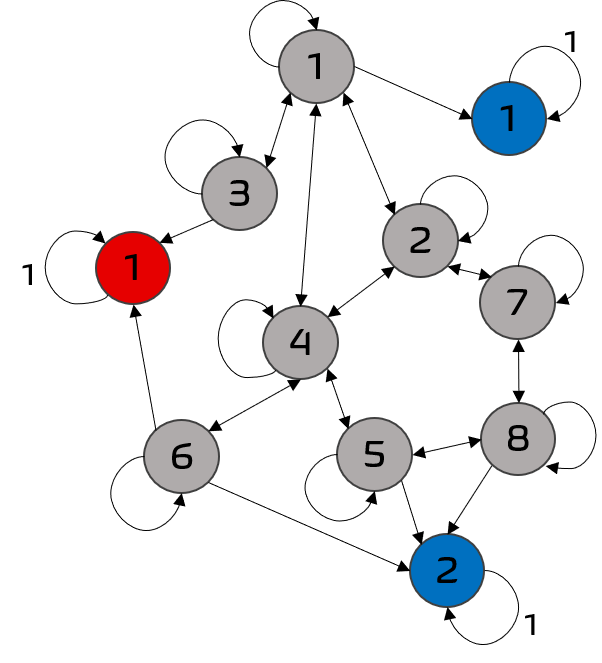
\includegraphics[width=2.5in]{Figures/network_example.png}
\caption{Example of one network that could be generated with our model. The directed graph is formed by eight individuals 1-8, one source of fake news (red), two sources of real news (blue), and links between nodes. Every node has a self loop, with weight 1 for the news sources, and the news sources only have in-neighbors.}
\label{pics:network_example}
\end{figure}
In order to be able to use a multitude of theoretical and analytical tools learned during the course, a linear model with the following update equation is studied
\begin{equation}
\label{eq:model}
x(k+1) = A x(k),
\end{equation}
where $x_i(k) \in [-1;1]$ represents the opinion of individual or source  $i$ at timestep $k$ and $A$ is the adjacency matrix of the network, as in the popular opinion model\cite{Friedkin1990}.
Constructing the adjacency matrix $A$ is a non-trivial task as it requires several assumptions on the the existence of links between people, the existence of links between people and news sources, and the importance of each such link.
The existence of links between different individuals and between individuals and sources is determined either by their physical distance or randomly, as will be explained in more detail in Subsection~\ref{subsec:connections_existence}.
To compute the weights in the adjacency matrix, several qualitative but sensible (in the authors' opinions) assumptions are made:
\acomment{spiegare: C, nRoot, local/non-local news connection}
\renewcommand{\theenumi}{\roman{enumi}}
\begin{enumerate}
\item \textit{Similarity}: connections between similar people are stronger. This derives from the fact that people tend to listen to their peers, friends and colleagues more than people that are completely different from them \cite{Youyou2017}\cite{Afifi2013}. Real-world concepts that define similarity may include, but are not limited to: career path, certain behavorial traits, age, nationality, etc.
\acomment{non funziona citazione}
\item \textit{Influenceability}: different people give different importance to their own personal opinions and can be more or less influenced by external opinions.
\item \textit{Critical thinking}: a person may believe \textit{news sources} more or less, depending on how developed the critical thinking ability  is.
\end{enumerate}
Mathematically, 
Translating these assumptions into a network adjacency matrix $A$ can be done in multiple ways. In this research we mainly present one way for different experiments\acomment{quali different experiments con la prima variante di modello}, and then a second slightly modified one to investigate opinion polarization. 
\subsection{Population Matrix}
To build a realistic network, there needs to be some different between individuals. To differentiate between them, a \textit{population matrix} $P \in {[0,1]}^{N \times t}$ is introduced, where $N$ is the number of individuals in the network and $t$ is the number characteristics defined for each person. In this research, $t=3$ and the chosen characteristics are: \textit{similarity}, \textit{influenceability} and \textit{critical thinking ability}. The position of an individual inside the matrix $P$ matters, as can be seen in Paragraph~\ref{subsub: connections}.
\subsection{News Sources}
The number of news sources in the model is an important parameter when creating the network. We define the number of real news sources $N_{\text{real}}$ and the number of fake news sources $N_{\text{fake}}$.
\subsection{Existence of Connections}
\label{subsec:connections_existence}
When generating the adjacency matrix, connections between individuals and news sources need to be created.
\subsubsection{Connections Between Individuals}
\label{subsub: connections}
Connections are created based on geographical distance. The real-world is simplified to a straight line with periodic boundaries. The connection between individuals $i$ and $j$ is created with probability 
\acomment{spiegare come viene creata A, param C, nroot, locality o no}

\begin{equation}
P(i,j) = \frac{C}{\sqrt[\text{nRoot}]{\vert i-j\vert}}
\end{equation}
where $C$ and $nRoot$ are tunable parameters that shape the probability distribution. $C$ linearly increases or decreases the probability of connections between neighbors, while $\text{nRoot}$ defines how quickly $P(i,j)$ decays as a function of $\vert i-j \vert$.

\subsubsection{Connections Between Individuals and Sources}
Each news source has a number of connections (the "Range" of a news source) given by $\text{Range} = 10\% (N)$, where $N$ is the number of individuals.
News sources are connected to individuals either \textit{locally} or \textit{non-locally}. 
\\If the new sources are connected locally, for each news source an individual is chosen (from a uniform distribution) and then this individual and its $\tilde{N}$ geographically closest individuals (on the straight line defined at the beginning of this subchapter) are connected to the news source.
\\If instead the news sources are connected non-locally, $\tilde{N}$ individuals are randomly selected (from a uniform distribution) and connected to the news source.
\\In our framework, locality and non-locality of news sources can be set independently for real news sources and fake news sources.



\subsection{Importance of Connections}
Once a connection is present, also the strength of the link needs to be defined.

\subsubsection{Connections Between Individuals}
The weights of the connections between individuals $i,j$ are modified depending on the people matrix. The weights $a_{ij}$ are modified sequentially for each couple of individuals $(i,j)$ in the following way:

\acomment{quando si parla di come inizializzare il personality vector?}
\begin{enumerate}
\item[\text{Step 1}] \textit{Similarity:} $a_{ij}^{\text{new}} = \dfrac{a_{ij}^{\text{old}}}{1 + \vert s_i - s_j\vert}$, with $ i \neq j$ and where $s_i$ is the similarity value of individual $i$. Each individual is assigned a value of the similarity index $s_i \in [0,1]$. 
\item[\text{Step 2}] \textit{Influenceability:} $a_{ii}^{\text{new}} = a_{ii}^{\text{old}}+10*\dfrac{a_{ii}^{\text{old}}}{1 + f_i}$, where $s_i$ is the influenceability value of individual $f_i$. The scaling factor $10$ was found empirically by trying to balance the effects of similarity and influenceability on the weights of A, for the baseline cases described in Section~\ref{sec:experiments}.
\end{enumerate}
The last weight update concerns the weights between individuals and sources, and is explained in~\ref{subsub:ind_sources}.


\subsubsection{Connections Between Individuals and Sources}
\label{subsub:ind_sources}
\begin{enumerate}
\item[\text{Step 3}] \textit{Critical thinking:}$a_{iz}^{\text{new}} = k_i$ for real news sources, and $a_{iz}^{\text{new}} = 1 - k_i$ for fake news sources, where $a_iz$ is the weight of the connection from individual $i$ to the news source $z$ and $k_i \in [0,1]$ is the critical thinking parameter of individual $i$. A high critical thinking parameters (close to $1$), will make the individual give a higher importance to true news sources, while a small parameter will give more importance to fake news sources.
\end{enumerate}
After sequentially applying Steps 1-3 as described above, $A$ is normalized along its rows to make it row-stochastic.
\section{Theoretical Analysis}
\subsection{General Considerations}
Without loss of generality, the labels of the nodes in the graph can be selected so that the indices referring to the fake/real news sources appear to be the last ones. Considering $n_{People}$ as the number of people in the network and $n_{Sources}$ as the number of fake and real news sources, the matrix A can be then partitioned as illustrated in the following:

$$
A = 
\begin{bmatrix}
	\tilde{A}_{n_{People} \times n_{People}} & \tilde{B}_{n_{People} \times n_{Sources}} \\
	0_{n_{Sources} \times n_{People}} & I_{n_{Sources} \times n_{Sources}} \\
\end{bmatrix} 
\quad
$$

Where $\tilde{A}$ describes the reciprocal human-human interactions and $\tilde{B}$ describes how people's opinions are directly affected by the sources. The zero and identity matrices below encode the fact that the sources' opinions are not changing over time. \newline
The matrix A is row-stochastic, which implies that $1_n$ is eigenvector of A with eigenvalue 1. The Gershgorin disk theorem tells that a row-stochastic matrix cannot have an eigenvalue with magnitude greater than one. By applying the theorem to the treated case, where each diagonal element is different from zero, it can be concluded that the only possible eigenvalue with magnitude equal to one is 1 itself. The following therefore holds for the spectrum of A (1 has algebraic multiplicity $n_{mult}$):
\begin{align*}
spec(A) \subset \{\mu \in \mathbb{C}^n,\ \mu_i = 1\ \forall i & \in \{1,..,n_{mult}\},\\
| \mu_i | < 1 \text{ otherwise}\}
\end{align*}
Because $\rho(A) = 1$, the matrix A cannot be stable but it is semi-stable iff $1 \in spec(A)$ is semi-simple. \newline
The randomness in the graph generation process do not allow to conclude much more deterministically. The properties of $\tilde{A}$ are of great importance to infer the system behavior. It is remarkable that with the proposed set up: N = 100 individuals and C = 0.2, nRoot = 4 (this fully describes the probabilistic model of the connections between a person and his neighbors, see previous chapter), $\tilde{A}$ describes a strongly-connected graph in 99.4$\%$ of the cases. This value was obtained after generating 10000 different networks. The graph is directed and a connection from node i to node j implies a connection from j to i but with different weights in general. The 0.6$\%$ represents therefore some pathological and unlikely cases where part of the network is completely disconnected from the rest. This could represent an isolated and separated society living in our simulated world. Since these cases are relevant for the aim of this project (the news spread in a connected society is studied), these cases were simply discarded. From now on, it can therefore be assumed that the graph describing the human-human interactions is strongly connected, meaning that the matrix $\tilde{A}$ is irreducible.\newline In the following, the steady state behavior of the discrete time averaging system 
$$
x(t+1) = Ax(t)
$$
is analyzed under various circumstances.
\subsection{$n_{Sources} = 0$}
If there are no sources, the matrix A = $\tilde{A}$ describes a strongly connected digraph. Each node has a self-cycle meaning that the single strongly connected component is acyclic. The graph is therefore strongly connected and acyclic, which implies that the matrix A describing it is primitive. This, together with the fact that A is row-stochastic, implies that A is semi-convergent and that the discrete-time averaging system convergences to consensus and namely to:
$$
x_{\infty} = (w^Tx(0))1_n = \left(\sum_{i=1}^{n_{People}}w_ix_i(0)\right)1_n
$$
$$
w^TA = w^T,\ 
Av = v,\ 
v \geq 0,\ w \geq 0,\ w^Tv = 1
$$
\subsection{$n_{Sources} >= 2$}
\begin{figure}[!t]
	\centering
	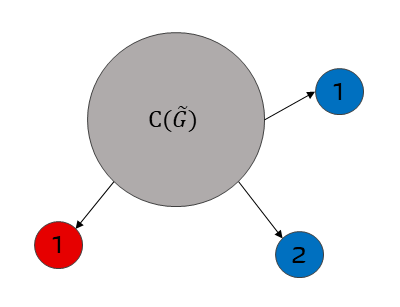
\includegraphics[width=2.5in]{Figures/condensation_digraph.png}
	\caption{Example of a network condensation digraph C(G). The people interactions are summarized as a single node, there are then one source of fake news (red) and two sources of real news (blue).}
	\label{pics:condensation_digraph_example}
\end{figure}
Figure~\ref{pics:condensation_digraph_example} shows an example condensation digraph for a network with irreducible $\tilde{A}$, one source of fake news and two sources of real news. The condensation is in general composed of $n_{Sources}+1$ nodes. The sources are all represented by sinks and the network of people by a single node connected to all sinks. \newline
All strongly connected components are furthermore acyclic: both the sources and the individuals have self-loops.
According to theorem 5.2 from the lecture notes, for a row-stochastic matrix A with multiple aperiodic sinks ($n_{Sources} \geq 2$), the following holds:
\begin{enumerate}
	\item
	A is semi-convergent.
	\item
	The eigenvalue 1 is semi-simple with multiplicity $n_{Sources}$ and all other eigenvalues $|\mu|<1$.
	\item
	The left eigenvectors $w^p \in \mathbb{R}^n$, $p\in \{1,...,n_{Sources}\}$, of A corresponding to the eigenvalue 1 can be selected to satisfy: $w^p\geq0,\ 1_n^Tw^p=1$, $w^p_i>0$ if and only if node i belongs to sink p.
	\item
	$
	x_{\infty}^i = 
	\begin{cases}
	(w^p)^Tx(0),& \text{node i $\in$ sink p}\\
	\sum_{p=1}^{n_{Sources}} z_{i,p}((w^p)^Tx(0)), & \text{otherwise}
	\end{cases}
	$
	where $z_{i,p},\ p\in\{1,...,n_{Sources}\}$, are convex combination coefficients and $z_{i,p} > 0$ if and only if there exists a directed path from node i to the sink p. This is always true for the individuals in this case making $z_{i,p} > 0\ \forall\ p \in \{1,...,n_{Sources}\}$ and $i \in \{1,...,n_{People}\}$.
\end{enumerate}
The third statement for the treated scenario implies $(w^p)^T = (0_{1 \times n_{People}},\ 0_{1 \times (p-1)},\ 1,\ 0_{1 \times (n_{Sources}-p)})$. This is because there is only one node in each sink p. The index referring to that node is therefore the only one different from zero in $w^p$. $1_n^Tw=1$ enforces its value to be exactly equal to 1. By plugging this result into iv), one can obtain the following:
$$
x_{\infty}^i = 
\begin{cases}
	x(0)^{n_{People}+p},& \text{node i $\in$ sink p}\\
	\sum_{p=1}^{n_{Sources}} z_{i,p}(x(0)^{n_{People}+p}), & \text{otherwise}
\end{cases}
$$
where $x(0)^{n_{People}+p}$ is the ($n_{People}+p$)th element of x(0). The steady state value of x therefore does not depend on the population initial conditions. It just depends on the sources'. Furthermore, it depends on $z_{i,p}$, whose value is strictly greater than zero for the population as  illustrated earlier. Their exact value depends on the random variables in our model and therefore cannot be estimated in general. (verificare) \newline
The result can be further simplified by plugging in the values of the initial conditions (-1 for fake and +1 for real news sources):
$$
x_{\infty}^i = 
\begin{cases}
\delta_p,& \text{node i $\in$ sink p}\\
\sum_{p=1}^{n_{Sources}} z_{i,p}\delta_p, & \text{otherwise}
\end{cases}
$$
where 
$
\delta_p = 
\begin{cases}
1,& \text{sink p is real news source}\\
-1,& \text{sink p is fake news source}
\end{cases}
$
$z_{i,p},\ p\in\{1,...,n_{Sources}\}$, are convex combination coefficients, which means that $\sum_{p=1}^{n_{Sources}} z_{i,p} = 1$ $\forall$ i.
If there is only one type of sources (either fake or real news), then $\sum_{p=1}^{n_{Sources}} z_{i,p}\delta = \delta*\sum_{p=1}^{n_{Sources}} z_{i,p} = \delta$ which is either +1 or -1 depending on whether the only type of source is real or fake: 
$x_\infty = 
\begin{cases}
1_n,& \text{Only real news sources}\\
-1_n,& \text{Only fake news sources}
\end{cases}$ 
\subsection{$n_{Sources} = 1$}
If $n_{Sources}=1$, then there is either a single fake or real news source. The condensation digraph contains a single aperiodic sink, which is composed by the source itself. The source is reachable from every node in G and the other nodes are reachable from every node in the graph but from the source. This makes the divulger the only globally reachable node in the graph. Its subgraph is furthermore aperiodic. From this it follows for the row-stochastic matrix A:
\begin{enumerate}
	\item
	The eigenvalue 1 is simple and all other eigenvalues $\mu$ satisfy $|\mu|<1$
	\item
	A is semi-convergent and $lim_{k->\infty} A^k = 1_n w^T$, where $w \in \mathbb{R}^n$ satisfies $w>=0, 1_n^T w = 1$, and $w^TA=w^T$
	\item
	$w>=0$ is the left dominant eigenvector of A and $w_i>0$ if and only if $i$ is globally reachable. As previously discussed, this is only the case for the single source in the treated example. \newline
	$\implies$ $w^T = (0,...,0,1)$.
	\item
	$x_\infty = (w^T x(0))1_n = x(0)^n 1_n = 	\begin{cases}
	1_n,& \text{Real news source}\\
	-1_n, & \text{Fake news source}
	\end{cases}$
	\newline The whole network would therefore converge to the source opinion for any people's initial conditions.
\end{enumerate}
\section{Introduction}

\section{Numerical Experiments}
\label{sec:experiments}

For the numerical experiments presented in this chapter, we define a baseline set up. In all experiments, if not differently specified, we keep all the parameters as in the baseline set up. 
The parameter values for these baselines are chosen with trial and error with the following goals:

\begin{itemize}
	\item
	Number of people sufficiently large in order not too have a too large variance over different experiments with same parameters.
	\item
	Reasonable computation time per experiment.
	\item
	Reasonable average number of connections per individual and avoiding cases with a non-strongly connected graph (see Chapter~\ref{sec:mathematical})
\end{itemize}


Table \ref{table:1} summarizes the parameter values for the baseline.
\begin{table}[h!]
\centering
\begin{tabular}{||c | c || c | c ||}
	\hline
	Parameter&Value&Parameter&Value\\
	\hline
	$C$&0.2&Range& $[ 0.1\ n_p,\ 0.1\ n_p]$\\
	nRoot&4&News con. type&$[Local,\ Local]$\\
	$n_p$&100&Similarity&$U(0,1)$\\
	$n_f$&2&Crit. Thinking&$U(0,1)$\\
	$n_r$&2&Influenceability&$U(0,1)$\\
	$x(0)$& $0_{n}$ & &\\
	\hline
\end{tabular}
\newline
\caption{Baseline parameter values. For Range and News connection type, the first component refers to the real news sources and the second component refers to the fake news sources. $U$ denotes the uniform random distribution.}
\label{table:1}
\end{table}


For the experiments where convergence is studied, the following expression was used to determine the steps to convergence $k_{\infty}:$
$$
k_{\infty}=\min k$$
such that
$$ \frac{1}{n_p} \sum_{j=1}^{n_p} \vert x(k+1)_j-x(k)_j \vert <  \tau
$$
where $\tau$ is the tolerance accepted for steady-state, here
$\tau = 0.0001$. In other words, the system is considered at convergence if the average opinion changes for each node is below $0.01\% $ with respect to the previous step.


\subsection{Instruction Level}
\label{sec:Instr_Level}
The goal of this section is to investigate the effect of the \emph{instruction level} on the population's steady state opinions. The instruction level $L \in [0,1]$ models the capacity of people to identify whether a source is spreading real or fake news. For this experiment, we will assume that the instruction level directly affects the trait \emph{critical thinking}. A function $f$  that maps an instruction level to its corresponding critical thinking probability distribution is defined as:
$$
f: L \to p 
$$
with
$$
p:= \{g,\ g: [0,1] \to \mathbb{R}_+,\ \int_{0}^{1} g(x) \,dx = 1\}.
$$
In order to obtain this mapping, the beta distribution is employed: 
$$
f(L) = \text{Beta}(\alpha(L), \beta(L))\ L \in [0,1]
$$
And therefore:
$$
P(CT_i\in[x,x+dx]) = [f(L)](x) dx \text{ with } x\in [0,1],
$$
where $CT_i$ is the critical thinking parameter for individual i. 
The relation between the parameters $\alpha$ and $\beta$ and the instruction level $L$ is given by: 
$$
\{\alpha, \beta\} = 
\begin{cases}
parity \times \{2^{factor},\ 1\},& \text{L $\geq$ 0.5}\\
parity \times \{1,\ 2^{factor}\},& \text{otherwise}
\end{cases}
$$
$$ 
\text{where }
\text{$parity$ = 1.3 and $factor$ = -(6 $\times$ $L$ - 3)}
$$
For L = 0, $\{\alpha, \beta\} = 1.3\times\{1,\ 8\}$, for L = 1, $\{\alpha, \beta\} = 1.3\times\{8,\ 1\}$ and for L = 0.5, $\{\alpha, \beta\} = 1.3\times\{1,\ 1\}$. The parameter $parity$ is the value, which both parameters take when the instruction level is mediocre (L = 0.5). The parameter $\alpha$ ($\beta$) grows as L increases (decreases) from 0.5, while $\beta$ ($\alpha$) stays the same. 
\begin{figure}[!t]
	\centering
	\subfloat[Instruction level = 0.1]{\label{a}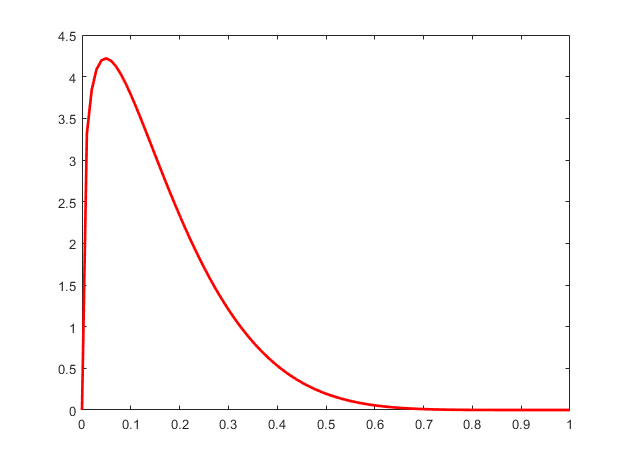
\includegraphics[width=.5\linewidth]{Figures/instr01.png}}\hfill
	\subfloat[Instruction level = 0.5]{\label{b}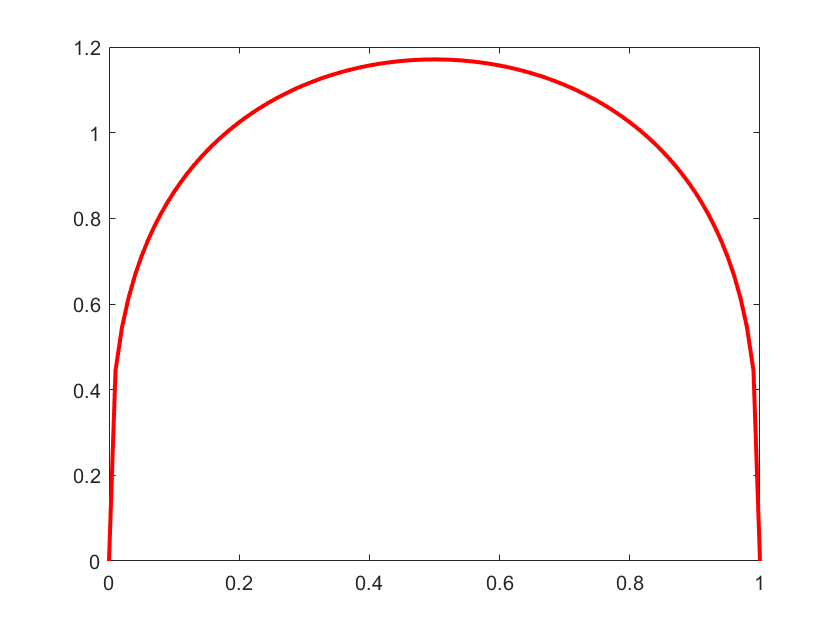
\includegraphics[width=.5\linewidth]{Figures/instr05.png}}\par 
	\subfloat[Instruction level = 0.9]{\label{c}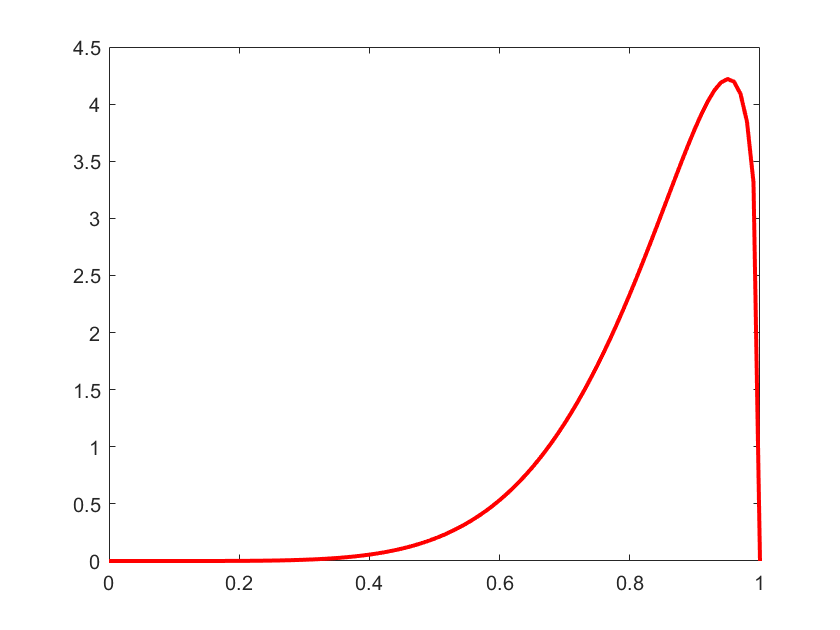
\includegraphics[width=.5\linewidth]{Figures/instr09.png}}
	\caption{Critical thinking probability distribution for instruction level = \{0.1, 0.5, 0.9\}.}
	\label{pics:critdistribution}
\end{figure}

Figure~\ref{pics:critdistribution} shows the critical thinking probability distribution for three examples of instruction level. A higher instruction level implies, on average, a more critical society with the distribution peak moving to the right (higher critical thinking coefficient). Vice versa, a low instruction level moves the distribution peak to the left (lower critical thinking coefficient). \newline

\begin{figure}[!t]
	\centering
	\subfloat[Average vs Intruction Level level]{\label{a}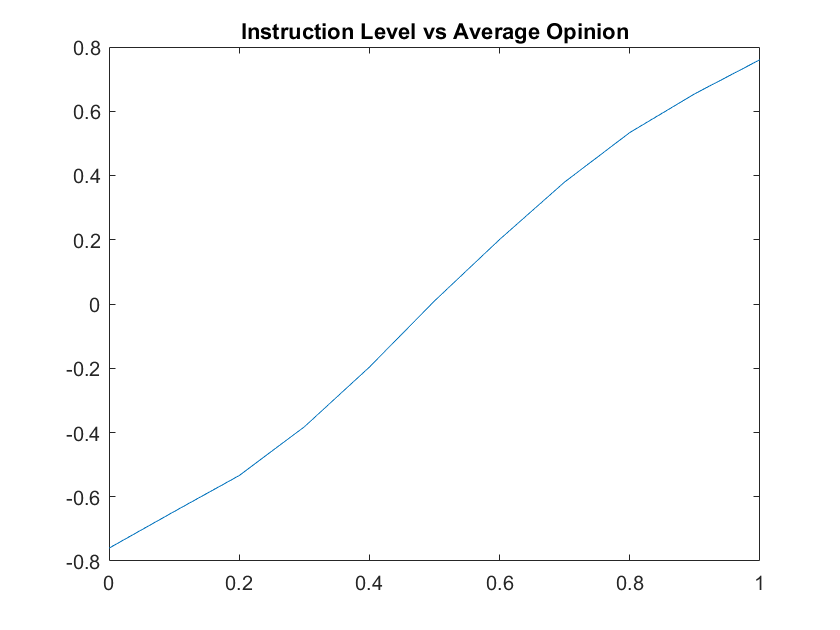
\includegraphics[width=.5\linewidth]{Figures/instruct_average.png}}\hfill
	\subfloat[Std vs Intruction Level]{\label{b}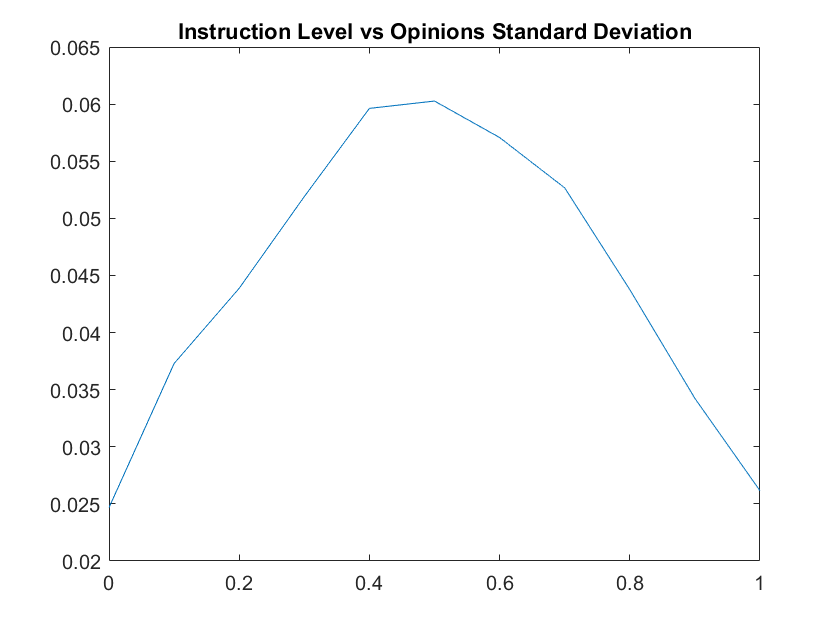
\includegraphics[width=.5\linewidth]{Figures/instruct_std.png}}\par 
	\caption{Average opinion and standard deviation of opinions for instruction level = 0:0.1:1.}
	\label{pics:critstatistics}
\end{figure}

In the experiments, the parameter instruction level is varied in its whole range [0,1] and the average opinion and the opinions' standard deviation are computed. The rest of the parameters are left as in Baseline. For each instruction level, 100 cases have been randomly generated and the average metrics have been computed for the steady state opinions.
Figure~\ref{pics:critstatistics} shows the results. As expected, the higher the instruction level, the closer the average opinion is to 1. Vice versa, the lower the instruction level, the closer the average opinion to -1. Furthermore, as the peak gets sharper (either on the right or on the left side) the standard deviation decreases. The opinion therefore converges to values close to 1 (or -1) and the standard deviation decreases as $|L-0.5|$ increases. 
\subsection{Society Diversity}
\label{sec:diversity}
The goal of the numerical experiment presented in this section is investigating the effect of the \textit{diversity factor} $D$ on the transient and steady state behavior of the network opinions. The parameter $D \in \mathbb{R}$ models the diversity of the individuals in the network and will therefore impact the trait \textit{similarity.}
The similarity trait $s_i$ for each individual is drawn from the uniform distribution between $-D$ and $D$:
$$
s_i \backsim U(-D, D),\ D \in \mathbb{R}
$$

The diversity in the society increases as $D$ increases and decreases as $D$ decreases. Each possible similarity value occurs with the same probability but as $D$ increases, the spectrum of possibilities gets larger. \newline
In the experiments, the parameter $D$ is varied in the range [0,50] and the average opinion and the opinions standard deviation are computed. Furthermore the length of the transient phase is recorded. The rest of the parameters are left as in Baseline. For each $D$, 100 networks have been randomly generated and the average metrics have been computed for the steady state opinions, the standard deviations and the time to convergence. 

\begin{figure}[!t]
	\centering
	\subfloat[Average vs Similarity level]{\label{a}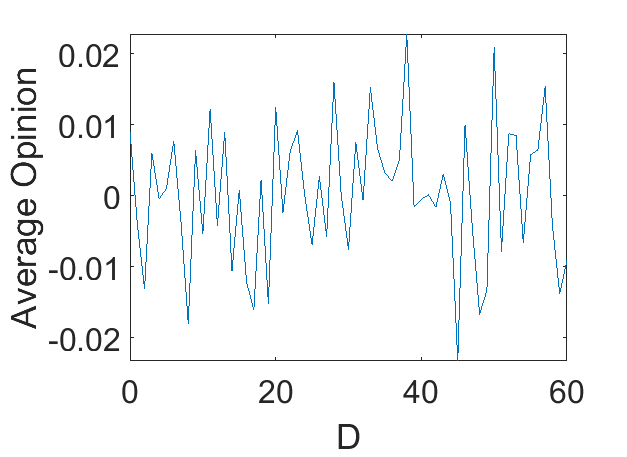
\includegraphics[width=.5\linewidth]{Figures/similarity_vs_average.png}}\hfill
	\subfloat[Std vs Similarity Level]{\label{b}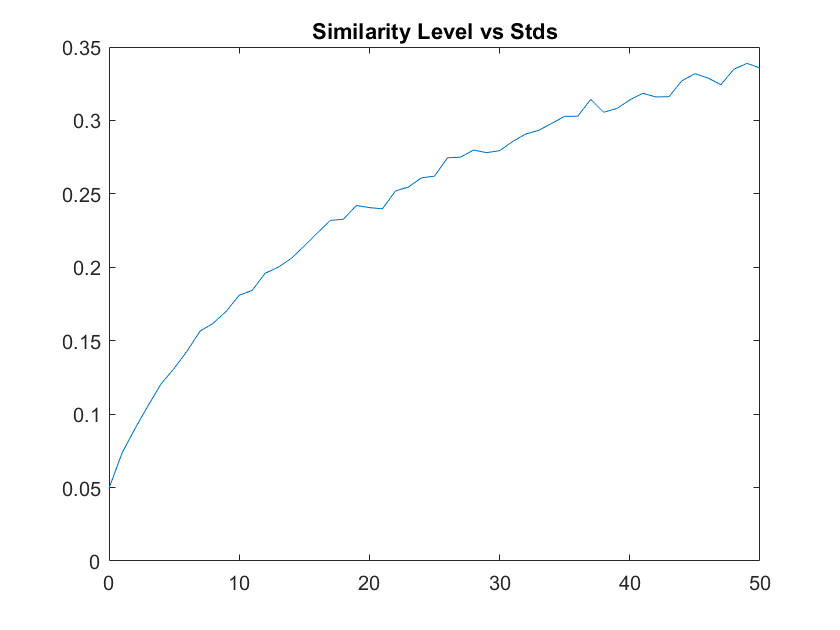
\includegraphics[width=.5\linewidth]{Figures/similarity_vs_std.png}}\par 
	\subfloat[Time to Steady State vs Similarity Level]{\label{c}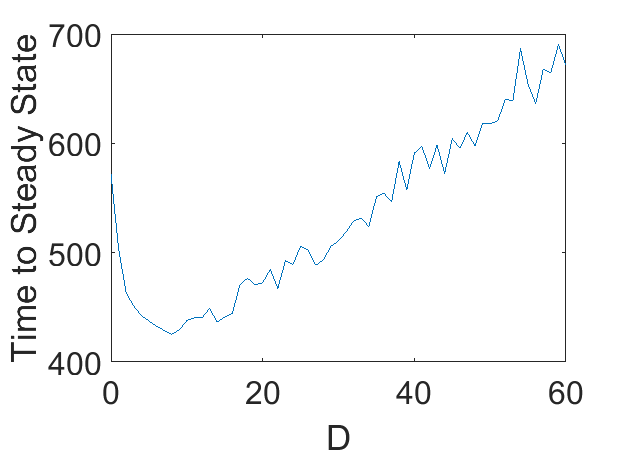
\includegraphics[width=.5\linewidth]{Figures/similarity_vs_timesteps.png}}
	\caption{Average opinion, standard deviation of opinions and time to steady state for $D$ = 0:1:50.}
	\label{pics:diversityresults}
\end{figure}
Figure~\ref{pics:diversityresults} illustrates the results. The average opinion does not show any trend as it oscillates with a small amplitude around the value zero, with no bias. This is explainable with the randomness of the network generation. The unbiasedness is expected since no opinion is preferred with this set up. By contrast, the standard deviation increases with $D$. This makes sense, since in a more diverse society, a wider range of opinions is expected. The steady state will therefore show a greater variety of opinions with the resulting larger standard deviation. Finally, the parameter time to steady state shows an initial decrease from $\approx$ 550 to $\approx$ 430 timesteps for $D \in [0,10]$ and then it starts increasing linearly with $D$. The linear increase can be explained by the fact that the weights between different individuals are smaller, and therefore the opinion propagation is slow.

\subsection{Population manipulability}
\label{sec:manipulability}
In this experiment, the goal is to investigate how modifying the \textit{influenceability} trait of the population affects the time to convergence of the opinions in the population. Qualitatively, this would be equivalent to study how well ideas spread in a "stubborn" population versus a highly manipulable population. If one thinks about the real world, the speed of idea spreading is a very important concept. A society with very stubborn individuals may be more stable, and on the other hand change is propelled by people with a flexible view on new ideas.
We define the \textit{manipulability level} $M \in [0,1]$ of the society and study how this affects the time to convergence of the opinion dynamics. A manipulability level of $0$ represents a society difficult to manipulate, while a manipulability level of $1$ represents a society where people are more influenceable. The mapping between $D$ and the population trait \textit{influenceability} is computed through the beta distribution, similarly to the mapping between $L$ and \textit{critical thinking} in Section~\ref{sec:Instr_Level}. For the numerical experiments, the manipulability level is varied in the range $[0,1]$ and the other parameters are left as in Baseline. The experiment is repeated 100 times and the results are averaged. A plot showing that the average time to steady state decreases when the society is more manipulable can be found in Figure~\ref{pics:man_steadystate}. In the range of $M\in [0,1]$, the time to steady state goes from around a maximum of $\approx 580$ timesteps to a minimum of $\approx 480$ timesteps. The result is in line with expectations: the less influenceable individuals are, and the larger weights of the self-loops in the graph will be. For individuals, this corresponds to favoring their own ideas instead of the neighbors' ones and "slowing" thus the information propagation in the network.
This result is in line with the comments made at the beginning of this section, i.e. that ideas spread faster in manipulable societies and slower in less manipulable societies.
\begin{figure}[!t]
	\centering
	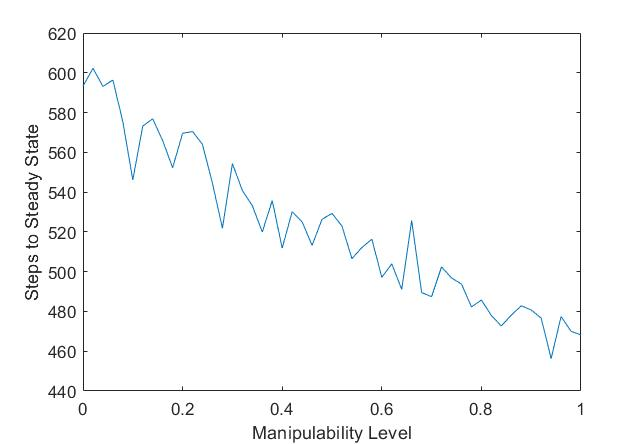
\includegraphics[width=3.5in]{Figures/exp8_final.jpg}
	\caption{Average timesteps necessary to reach steady state while varying the manipulability level in the range $[0,1]$.}
\label{pics:man_steadystate}
\end{figure}


\subsection{Polarization}
\label{sec:polarization}
The goal of the numerical experiments presented in this section is investigating the opinion polarization within a population using our model. In particular, we aim to understand how the model parameters influence the polarization. 
Polarization refers either to a distribution of opinions with multiple local maxima or to the process by which such strong divergences of opinions that divide a population come about \cite{Banisch2019}\cite{Bramsona2016}. The model presented in Chapter~\ref{sec:mathematical} has been slightly modified for what concerns the weights between individuals. If $s_i$ denotes the similarity trait of individual $i$, then, at $(S1)$ presented in Section~\ref{sec:conn_ind}, the entry $a_{ij} = a_{ji}$ is 
$$
a_{ij} = \text{max}\{0, \delta_{ij} + 0.2\ r\}
$$
where $r$ is a random number from the normal distribution $\mathcal{N}(0,1)$ and $\delta_{ij} = 1$ if $s_i = s_j$ otherwise $\delta_{ij} = 0$.

The number of real and fake sources is 3. The influenceability and critical thinking traits are set to $0.5$ for all individuals. Similarity is set to $1$ for the first half of individuals in the vector $x$ and to $0$ for the second half. Thus, the probability of creating a link remains the same, but the weight that the link has is around 1 if the nodes belong to the same half and non-negative and close to 0 if they belong to different halves. An example of a single experiment is shown in Figure~\ref{pics:exp20}.\\

\begin{figure}[!t]
\centering
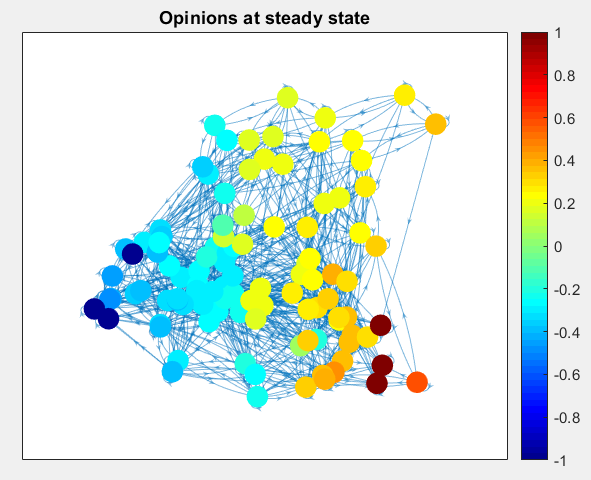
\includegraphics[width=8cm]{Figures/Exp20_graphb.png}
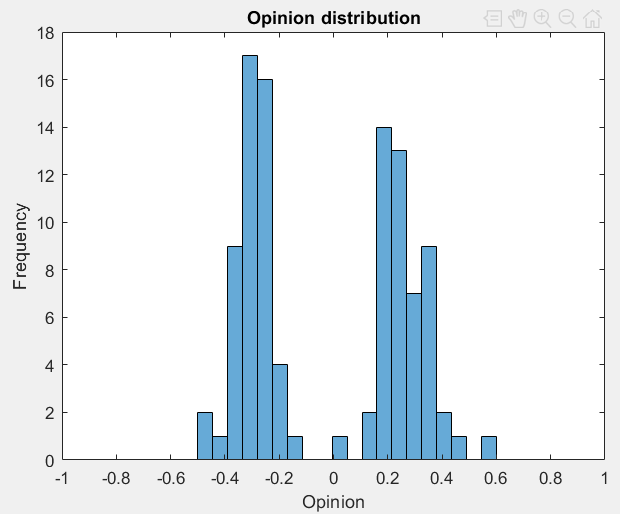
\includegraphics[width=8cm]{Figures/Exp20_hystb.png}
\caption{Simulation with 100 individuals, 3 sources of Fake and 3 of Real News, $C=0.2$, nRoot$=4$ and new connection local. Above: graph at steady state. Below: opinion distribution at steady sate.}
\label{pics:exp20}
\end{figure}

To the best of our knowledge, there is not a unique metric to quantify opinion polarization. We analyzed three metrics: the measure proposed in \cite{Matakos2017} defined as $R_2 = ||x_{\infty}||^2/ N$, the standard deviation of $x_{\infty}$ according to the interpretation of polarization as dispersion exposed in \cite{Bramsona2016} and the mean.\\

In our experiments, we varied three parameters: $C$ in the range $[0.2; 0.6]$, nRoot in the range $[2; 8]$ and the news connection type, which is either local or non-local. For each parameters combination, 100 cases have been randomly generated and the average metrics have been computed for the opinion vector at steady state.\\

The mean is at  $0 \pm 5\times 10^{-3}$ for all cases, which means that there is not a predominant opinion. This is expected, because the parametrization of the personality traits does not favour one opinion. When the news sources have non-local connections, the average is even closer to 0 ($0 \pm 10^{-3}$). Although in this section we are not interested in the average opinion, the fact that the mean is close to 0 supports the choice of using standard deviation and $R_2$ as metrics to evaluate the polarization. A high standard deviation correspond to many entries far from the center on both sides of the opinion spectrum.\\

Because of the mean $\overline{x}$ close to 0 and $N=100$, we have
$$ \sigma^2 = \frac{1}{N-1} \sum_{i=1}^N (x_i-\overline{x})^2 \approx \frac{1}{N} \sum_{i=1}^N x_i^2 = R_2.$$

Thus, the two metrics carry the same information about the polarization and, for the sake of simplicity, we only discuss the standard deviation. Results for 30 parameters combinations are shown in Figure~\ref{pics:pol_std}. Since the opinions are between $-1$ and $1$, the standard deviation is between 0 and 1.\\

We notice that the higher $C$ and nRoot are, the less polarized are the opinions. Moreover, the lower nRoot is, the faster the polarization grows by decreasing $C$. This is in line with our expectations. The higher $C$ is, the more likely contacts are, because $C$ is proportional to the average in and out degree of each node. A high nRoot means that each individual is more likely to have a link with another individual which is far and, in this case, contacts among individuals with different similarity are more likely. Thus, the experiments show that polarization arises in the society when individuals are in contact with few other people or when they are in contact mainly with similar people. The strongest polarization is present when both conditions are met.\\

\begin{figure}
\centering
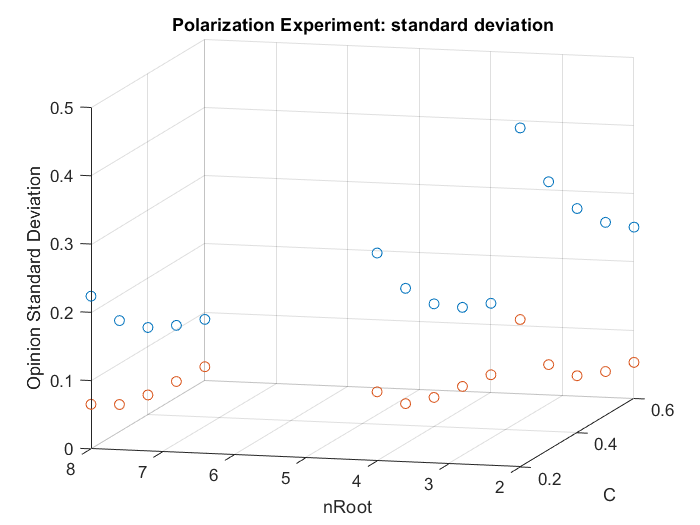
\includegraphics[width=8cm]{Figures/pol_std1.png}
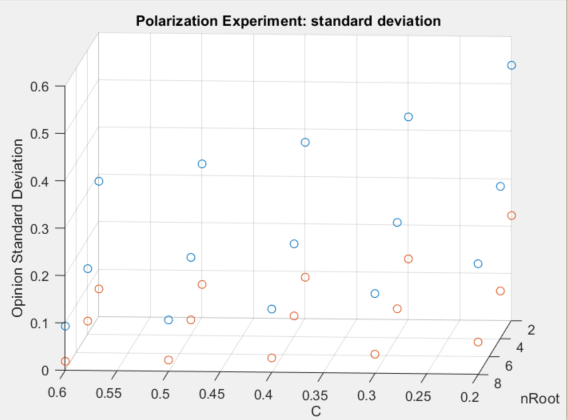
\includegraphics[width=8cm]{Figures/pol_std2.png}
\caption{Standard deviation for different combinations of C, nRoot and news connection. Red: news are spread. Blue: news are local.}
\label{pics:pol_std}
\end{figure}


Another remarkable result is the comparison between the cases where the news connection type is local (blue) and when it is non-local (red). Non-local news connectivity reduces the polarization in the network. This is in line with \cite{Lee2014a}.
For each $C$ and nRoot combination, the standard deviation is at most one third of the value for the corresponding case with local news connectivity. Also with non-local news connectivity, we observe an increase of polarization when $C$ and nRoot decrease, but the growth is less strong. This experiment suggests that a society where each individual has the chance to come in touch with all news sources and not only the ones close to their milieu, is less likely be polarized.


\section{Conclusion}
We started this work by motivating why the study of information spread in a society is so important, and came up with a simplified society where such spread could be studied. Here, the influence of several personality traits of the population's individuals, and the presence of real and fake news sources was studied. Our model has a linear update equation, which allows to use a lot of theoretical tools for analysis purposes. The model has a flexible implementation, which allows to test many different scenarios and even to make the society more complex by adding personality traits.
Numerical experiments were used to validate our model. In Section~\ref{sec:Instr_Level}, the average instruction level is varied and it is shown that this helps mitigate the spread of fare news. In Section~\ref{sec:diversity}, it is shown that in a diverse society, a broader spectrum of ideas have a place to exist. In a society where individuals are easily manipulable, as shown in Section~\ref{sec:manipulability}, ideas spread more rapidly than if the individuals are less manipulable.
Finally, in Section~\ref{sec:polarization} we propose a slightly modified model where we build a society in such a way that it is divided in two main groups, and show that this leads to polarization of ideas.\\
As mentioned, our model is simple but powerful, as it is built in such a way that it is expandable. Future work could focus on including new personality traits, or modifying how the weights are generated based on the defined personality traits. Another realistic addition to the model could be to give a different strength to news sources, i.e. make them more or less connected and with larger or smaller weights connecting them to the individuals.
Furthermore, focus  could be put on developing the algorithm that creates connections between individuals, to create different community structures. Finally, the model could be extended to include also non-constant adjacency matrices to capture more effects of the opinion spread, such as perturbations or active control on the system. 
 

\newpage
\appendix
\section{Introduction}


\end{document}
